\documentclass{standalone} 
         \usepackage{graphicx} 
 \usepackage[hang,small,bf]{caption}    % fancy captions
 \usepackage{tikz}	

% TikZ libraries 
\usetikzlibrary{shapes,snakes} 
\usetikzlibrary{backgrounds,fit,decorations.pathreplacing} 
 \usetikzlibrary{shapes,arrows,fit,calc,positioning,automata} 
\newcommand{\ket}[1]{\ensuremath{\left|#1\right\rangle}} % Dirac Kets 
\begin{document} 
    %\begin{figure} 
    %\centerline{ 
        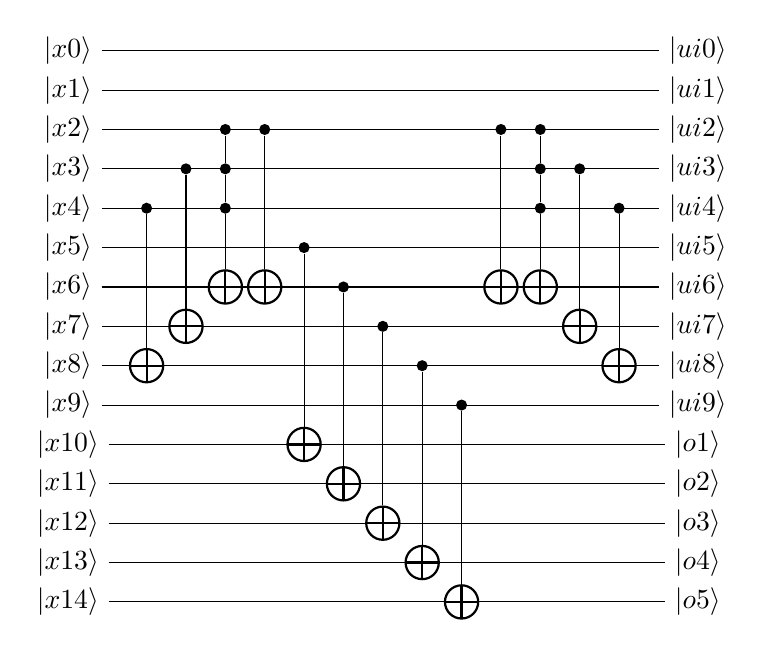
\begin{tikzpicture}[] 
            \tikzset{oplus/.style={path picture={% 
            \draw[black] 
            (path picture bounding box.south) -- (path picture bounding box.north) 
            (path picture bounding box.west) -- (path picture bounding box.east);
            }}}
             \tikzstyle{operator} = [draw,fill=white,minimum size=1.5em] 
             \tikzstyle{phase} = [fill,shape=circle,minimum size=4pt,inner sep=0pt]
             \tikzstyle{surround} = [fill=blue!10,thick,draw=black,rounded corners=2mm]
             \tikzstyle{swap} = [draw,fill,shape=cross out,minimum size=5pt,inner sep=0pt]
             \tikzstyle{cnot} = [oplus,draw,thick,circle,minimum size = 12pt]		% Qubit
		\node at (0,-0.0)(q0_0) {\ket{x0}};
		\node at (0,-0.5)(q0_1) {\ket{x1}};
		\node at (0,-1.0)(q0_2) {\ket{x2}};
		\node at (0,-1.5)(q0_3) {\ket{x3}};
		\node at (0,-2.0)(q0_4) {\ket{x4}};
		\node at (0,-2.5)(q0_5) {\ket{x5}};
		\node at (0,-3.0)(q0_6) {\ket{x6}};
		\node at (0,-3.5)(q0_7) {\ket{x7}};
		\node at (0,-4.0)(q0_8) {\ket{x8}};
		\node at (0,-4.5)(q0_9) {\ket{x9}};
		\node at (0,-5.0)(q0_10) {\ket{x10}};
		\node at (0,-5.5)(q0_11) {\ket{x11}};
		\node at (0,-6.0)(q0_12) {\ket{x12}};
		\node at (0,-6.5)(q0_13) {\ket{x13}};
		\node at (0,-7.0)(q0_14) {\ket{x14}};
		% Gate 1
		\node[phase] (q1_4) at (1.0,-2.0) {} edge [-] (q0_4);
		\node[cnot] (q1_8) at (1.0,-4.0) {} edge [-] (q0_8);
		\draw[-] (q1_4)  -- (q1_8);
		% Gate 2
		\node[phase] (q2_3) at (1.5,-1.5) {} edge [-] (q0_3);
		\node[cnot] (q2_7) at (1.5,-3.5) {} edge [-] (q0_7);
		\draw[-] (q2_3)  -- (q2_7);
		% Gate 3
		\node[phase] (q3_2) at (2.0,-1.0) {} edge [-] (q0_2);
		\node[phase] (q3_3) at (2.0,-1.5) {} edge [-] (q2_3);
		\node[phase] (q3_4) at (2.0,-2.0) {} edge [-] (q1_4);
		\node[cnot] (q3_6) at (2.0,-3.0) {} edge [-] (q0_6);
		\draw[-] (q3_2)  -- (q3_3);
		\draw[-] (q3_3)  -- (q3_4);
		\draw[-] (q3_4)  -- (q3_6);
		% Gate 4
		\node[phase] (q4_2) at (2.5,-1.0) {} edge [-] (q3_2);
		\node[cnot] (q4_6) at (2.5,-3.0) {} edge [-] (q3_6);
		\draw[-] (q4_2)  -- (q4_6);
		% Gate 5
		\node[phase] (q5_5) at (3.0,-2.5) {} edge [-] (q0_5);
		\node[cnot] (q5_10) at (3.0,-5.0) {} edge [-] (q0_10);
		\draw[-] (q5_5)  -- (q5_10);
		% Gate 6
		\node[phase] (q6_6) at (3.5,-3.0) {} edge [-] (q4_6);
		\node[cnot] (q6_11) at (3.5,-5.5) {} edge [-] (q0_11);
		\draw[-] (q6_6)  -- (q6_11);
		% Gate 7
		\node[phase] (q7_7) at (4.0,-3.5) {} edge [-] (q2_7);
		\node[cnot] (q7_12) at (4.0,-6.0) {} edge [-] (q0_12);
		\draw[-] (q7_7)  -- (q7_12);
		% Gate 8
		\node[phase] (q8_8) at (4.5,-4.0) {} edge [-] (q1_8);
		\node[cnot] (q8_13) at (4.5,-6.5) {} edge [-] (q0_13);
		\draw[-] (q8_8)  -- (q8_13);
		% Gate 9
		\node[phase] (q9_9) at (5.0,-4.5) {} edge [-] (q0_9);
		\node[cnot] (q9_14) at (5.0,-7.0) {} edge [-] (q0_14);
		\draw[-] (q9_9)  -- (q9_14);
		% Gate 10
		\node[phase] (q10_2) at (5.5,-1.0) {} edge [-] (q4_2);
		\node[cnot] (q10_6) at (5.5,-3.0) {} edge [-] (q6_6);
		\draw[-] (q10_2)  -- (q10_6);
		% Gate 11
		\node[phase] (q11_2) at (6.0,-1.0) {} edge [-] (q10_2);
		\node[phase] (q11_3) at (6.0,-1.5) {} edge [-] (q3_3);
		\node[phase] (q11_4) at (6.0,-2.0) {} edge [-] (q3_4);
		\node[cnot] (q11_6) at (6.0,-3.0) {} edge [-] (q10_6);
		\draw[-] (q11_2)  -- (q11_3);
		\draw[-] (q11_3)  -- (q11_4);
		\draw[-] (q11_4)  -- (q11_6);
		% Gate 12
		\node[phase] (q12_3) at (6.5,-1.5) {} edge [-] (q11_3);
		\node[cnot] (q12_7) at (6.5,-3.5) {} edge [-] (q7_7);
		\draw[-] (q12_3)  -- (q12_7);
		% Gate 13
		\node[phase] (q13_4) at (7.0,-2.0) {} edge [-] (q11_4);
		\node[cnot] (q13_8) at (7.0,-4.0) {} edge [-] (q8_8);
		\draw[-] (q13_4)  -- (q13_8);
		% Output
		\node at (8.0,-0.0)(q14_0) {\ket{ui0}};
		\draw[-] (q0_0)  -- (q14_0);
		\node at (8.0,-0.5)(q14_1) {\ket{ui1}};
		\draw[-] (q0_1)  -- (q14_1);
		\node at (8.0,-1.0)(q14_2) {\ket{ui2}};
		\draw[-] (q0_2)  -- (q14_2);
		\node at (8.0,-1.5)(q14_3) {\ket{ui3}};
		\draw[-] (q0_3)  -- (q14_3);
		\node at (8.0,-2.0)(q14_4) {\ket{ui4}};
		\draw[-] (q0_4)  -- (q14_4);
		\node at (8.0,-2.5)(q14_5) {\ket{ui5}};
		\draw[-] (q0_5)  -- (q14_5);
		\node at (8.0,-3.0)(q14_6) {\ket{ui6}};
		\draw[-] (q0_6)  -- (q14_6);
		\node at (8.0,-3.5)(q14_7) {\ket{ui7}};
		\draw[-] (q0_7)  -- (q14_7);
		\node at (8.0,-4.0)(q14_8) {\ket{ui8}};
		\draw[-] (q0_8)  -- (q14_8);
		\node at (8.0,-4.5)(q14_9) {\ket{ui9}};
		\draw[-] (q0_9)  -- (q14_9);
		\node at (8.0,-5.0)(q14_10) {\ket{o1}};
		\draw[-] (q0_10)  -- (q14_10);
		\node at (8.0,-5.5)(q14_11) {\ket{o2}};
		\draw[-] (q0_11)  -- (q14_11);
		\node at (8.0,-6.0)(q14_12) {\ket{o3}};
		\draw[-] (q0_12)  -- (q14_12);
		\node at (8.0,-6.5)(q14_13) {\ket{o4}};
		\draw[-] (q0_13)  -- (q14_13);
		\node at (8.0,-7.0)(q14_14) {\ket{o5}};
		\draw[-] (q0_14)  -- (q14_14);
		\end{tikzpicture} 
   %}
%\end{figure}
\end{document}
